\section{Inclusive Charged Current Event Analysis}
\label{sec:InclusiveAnalysis}

The muon neutrino beam produced at J-PARC passes through the 
off-axis ND280 detector. 
These neutrinos can interact via Charged Current (CC) 
or Neutral Current with the detector material. 
The CC interactions 
%are expected to 
will 
produce a $\mu^-$ track 
which will contain most of the time the majority of 
the incident neutrino momentum. \\
The analyses strategy is to search for 
the highest momentum negative track in an event 
and to tag it as the muom candidate track and the while  
%tag the 
event as 
%which simplifies the identification and tagging of  
a CC interaction one.
We note that 
the beam spill delivered by the J-PARC facility  
to the experiment has a sub-structure of bunches which are 
separated by beam dead-time. 
All analyses described in this document were done 
at the beam bunch level instead of the ND280-DAQ event (beam spill level).

\subsection{Event Selection}
\label{sec:SelectionFlow}

The CC inclusive selection procedure includes the main levels of 
information available (accelerator/near-complex level, 
track level, bunch level) 
which 
%includes three main steps that
are listed below:
\begin{itemize}
\item 
%Beam and Data Quality selection cuts:\\
%Each Spill quality is checked to have both quality:
Accelerator/Near-Complex level selection:\\
A spill is use for analysis only if the below quality checks are satisfied
\begin{itemize}
\item 
The beam/accelerator flag `GoodSpillFlag' is set to the value one
\item
The near detector-complex Data-Quality flag `ND280OffFlag' is equals to zero
\end{itemize}
\item 
%Track level selection cuts: \\
Track level selection: \\
The Tracker-to-\p0d matching algorithm, which is outlined 
in Sec. \ref{sec:MatchingAlgorithm}, is applied. 

The algorithm inputs are the available \p0d and Tracker tracks in a spill 
and its outputs are a set of 
%all the 
tracks that originate in the \p0d \footnote{These will include tracks that 
started at the edges of the \p0d i.e. passing through tracks.}
 and continued to pass through TPC1/Tracker sub-detector.

To note is that the algorithm will match uniquely any \p0d/Tracker track 
with the nearest Tracker/\p0d track 
(by $\Delta R$, see Sec. \ref{sec:MatchingAlgorithm}). 
%
%In each spill, we match together reconstructed tracks from TPC1/Tracker 
%and \p0d using the matching algorithm outlined in Section \ref{sec:MatchingAlgorithm}. As all of the track quality cuts have already been made at the matching stage, we only need a few more selection steps. These tracks must:

\item 
Bunch level selection:\\
All the output tracks from the previous stage are sorted into 
predefined bunch time windows (See Table \ref{tab:BunchTimeWindowsProd5}). 

Then from each active bunch we identify the muon candidate track 
and tag that event as a CC interaction.

A track is considered as the muon candidate if it satisfied 
all the requirements below.

\begin{itemize}
\item 
The candidate track charge is negative \\
(by the matched Tracker track charge property).
\item 
The candidate track begins in the \p0d volume\\ 
($-988\ mm< X <910\ mm$, $-1020\ mm< X <1010\ mm$, $-3139\ mm< X <-900\ mm$). 
This condition is required to reject external sources tracks   
(cosmic, magnet or sand interactions) while keeping the largest 
volume of the \p0d detector as a target. 
\item 
The candidate track momentum at the start of the track is the highest 
in that bunch.
\end{itemize}

%Then in final step the algorithm identifies in each bunch the highest momentum 
%candidate pair track and tags it as the muon candidate.
Finlay, only the muon candidate tracks which originated from 
inside the \p0d Water-Target FV (see Sec. \ref{sec:WTFV}) 
are accounted for the final results. 
\end{itemize}

\subsubsection{The \p0d Water Target Fiducial Volume}
\label{sec:WTFV}

The Water-Target (WT) Fiducial Volume (FV) cut used in this document  
is based on the FV description given in T2K-TN-073. 
The choice of the FV in the X and Y directions 
is made to minimize the uncertainty of the amount of water in the \p0d. 
In the Z direction, the FV corresponds to the water target region only. 
This also minimizes the physics uncertainty arising from 
the lead radiator sheets in the ECal super-\p0dules that 
are on the upstream and downstream ends of the water target. 
The FV values utilized in this note are summarized in Table \ref{tab:WTFV}.

\begin{table}[h]
\centering
\begin{tabular}{ccccc}
\toprule
Minimum & & & & Maximum \\
\hline
 -836 & $<$ & X & $<$ & 764 \\
 -871 & $<$ & Y & $<$ & 869 \\
 -2969 & $<$ & Z & $<$ & -1264 \\
\bottomrule
\end{tabular} 
\caption{The \p0d Water-Target Fiducial Volume used in the analyses, 
taken from Ref. \cite{tn73}}
\label{tab:WTFV} 
\end{table}

\subsubsection{Bunch Time Windows}
\label{sec:BunchTimeWindow}

%As 
The beam spill substructure is not the same for the different 
beam run periods, we have studied the track timing 
for Run 1-4 % and Run 2
for both Data and MC samples.
These studies have revealed a number of points that 
had to be addressed by our bunch time window determination 
and are listed here.
\begin{itemize}
\item
Run 1 has six bunches in each beam spill 
while Run 2 - 4 have eight bunches in each beam spill.
\item
Run 2 includes a bunch time shift that was introduced at January 2011 
(see Fig. \ref{fig:TrackTime}).
\item
The MC samples have the same six/eight 
bunch structure as the Data samples but their bunches (means) 
are shifted on average $\sim$250 ns from the data ones.
\end{itemize}

\begin{figure}
\centering
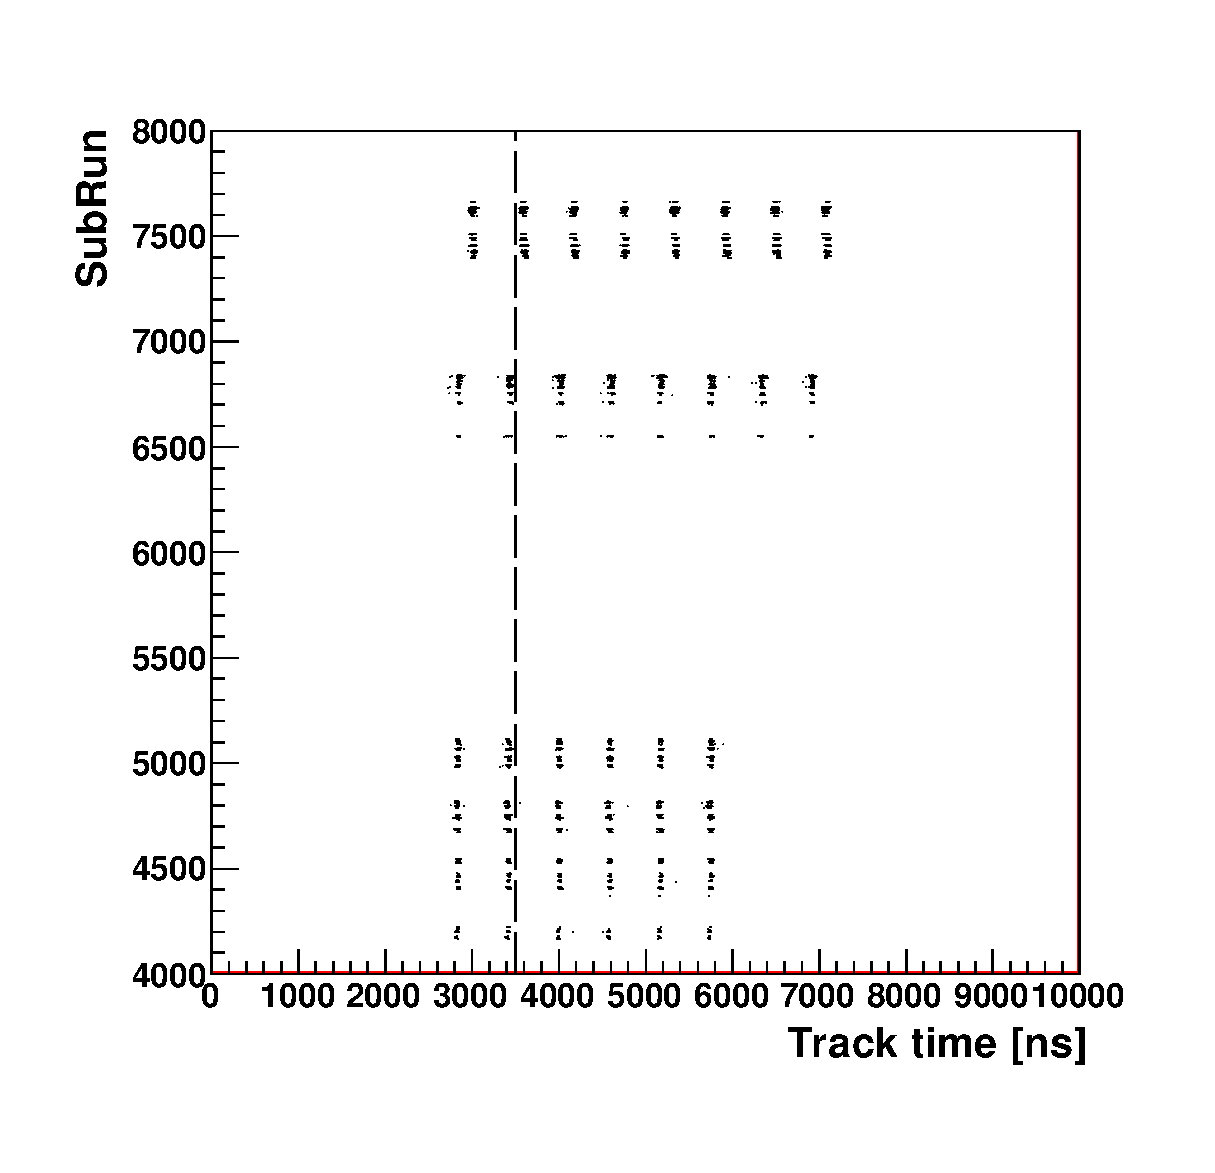
\includegraphics[width=4in]{Figures/spinD-TimeInSpill.eps}
\caption{Track time stamp as a function of subrun in Data 
(for Run 1 and Run 2 run periods). 
The vertical dash 
line was added to help point out the time shift that was introduced 
at Jan 2011.}
\label{fig:TrackTime}
\end{figure}

In Fig. \ref{fig:TrackTime}, 
which shows the track time stamps as a function of their subrun in Data, 
one can observe some of these effects mentioned above. 
A close examination of the figure shows 
both the six and the eight bunch structures 
and the time shift introduced at Jan 2011. 
A vertical dashed line was added to help the reader 
to help see this relative shift. \\

To account for the above conditions, we have decided to define 
the same set of bunch time windows for all runs periods 
(regardless of the run configuration).  
These windows were enlarged to include both the difference between 
Data and MC bunch means and the time shift in Run 2. 
Table \ref{tab:BunchTimeWindowsProd5} summarizes the 
bunch time windows used in the analyses. 

\begin{table}
\centering
\begin{tabular}{cc}\toprule
Bunch Number & Time window [ns]\\
\hline
 1 & 2660 - 3100\\ 
 2 & 3240 - 3680\\ 
 3 & 3820 - 4260\\ 
 4 & 4400 - 4840\\ 
 5 & 4980 - 5420\\ 
 6 & 5580 - 6000\\ 
 7 & 6140 - 6580\\ 
 8 & 6720 - 7160\\ 
\bottomrule
\end{tabular} 
\caption{The bunch timing windows used in the analyses 
for all Run periods.}
\label{tab:BunchTimeWindowsProd5} 
\end{table}

\clearpage

\subsection{Distributions and Selection Results}

In this section we present comparisons between data and Monte Carlo
for timing distributions, vertex distributions, momenta, $\theta$, and $\phi$. 
The Monte Carlo was reweighted to the 11b version 3.2 flux. The stacked color histograms in the following plots represent the MC distributions separated into different classifications. The color scheme used is shown in Figure \ref{fig:colorlegend}. Note that Quasi-elastic (QE), Single pion (Pi), Multi Pion (NPi), Meson, and Deep Inelastic Scattering (DIS) are all charged current interactions and are considered as signal in this analysis. Neutral Current (NC), parent Anti-Neutrino (antiNu), Other and Out of Fiducial Volume (outFV) interactions are all background.

\begin{figure}[here]
\centering
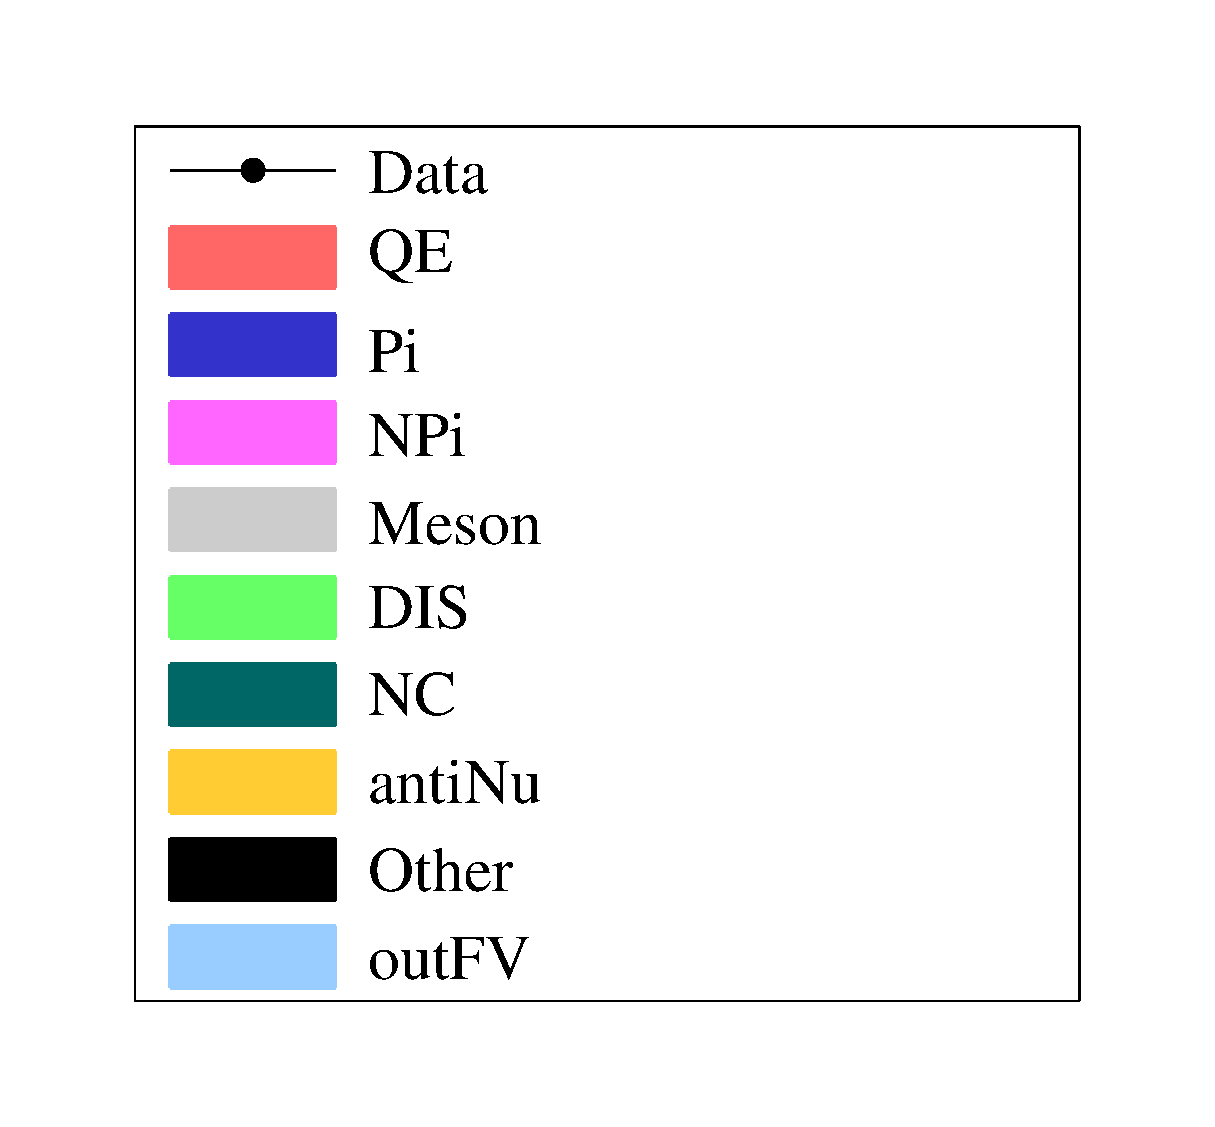
\includegraphics[width=3in]{Figures/Legend.eps}
\caption{The color scheme used for many of the Monte Carlo plots in the document. They are separated via NEUT reaction codes, parent neutrino flavor and vertex location. Refer to the text for further detail.}
\label{fig:colorlegend}
\end{figure}

\subsubsection{Timing distributions}

\begin{figure}[here]
\centering
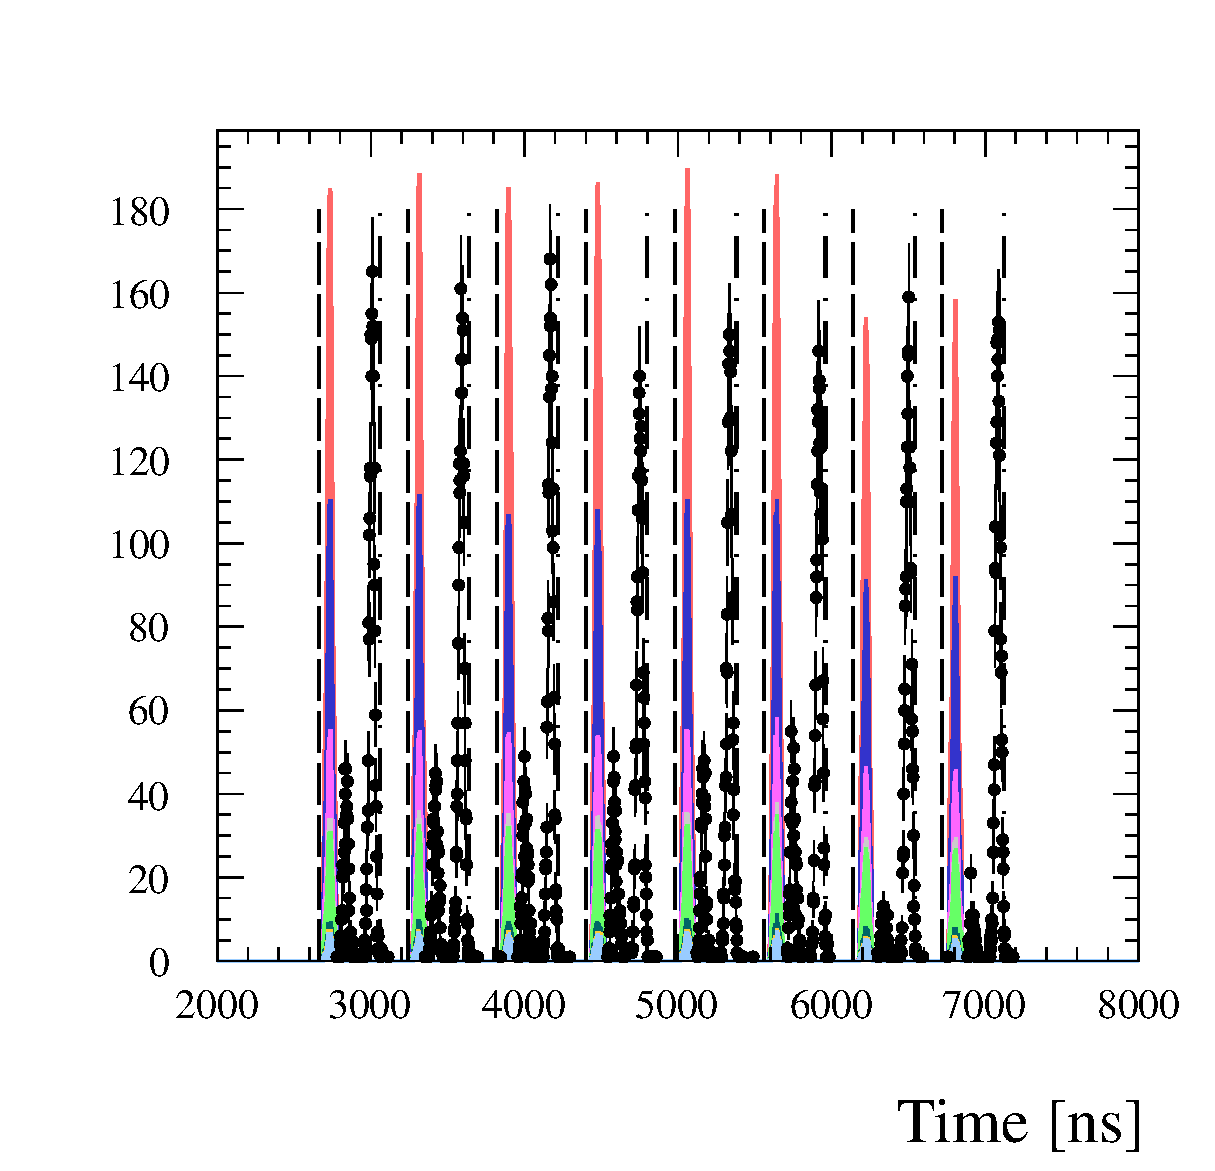
\includegraphics[width=3in]{Figures/P0DTrkTimeRun1Run2Run4.eps}
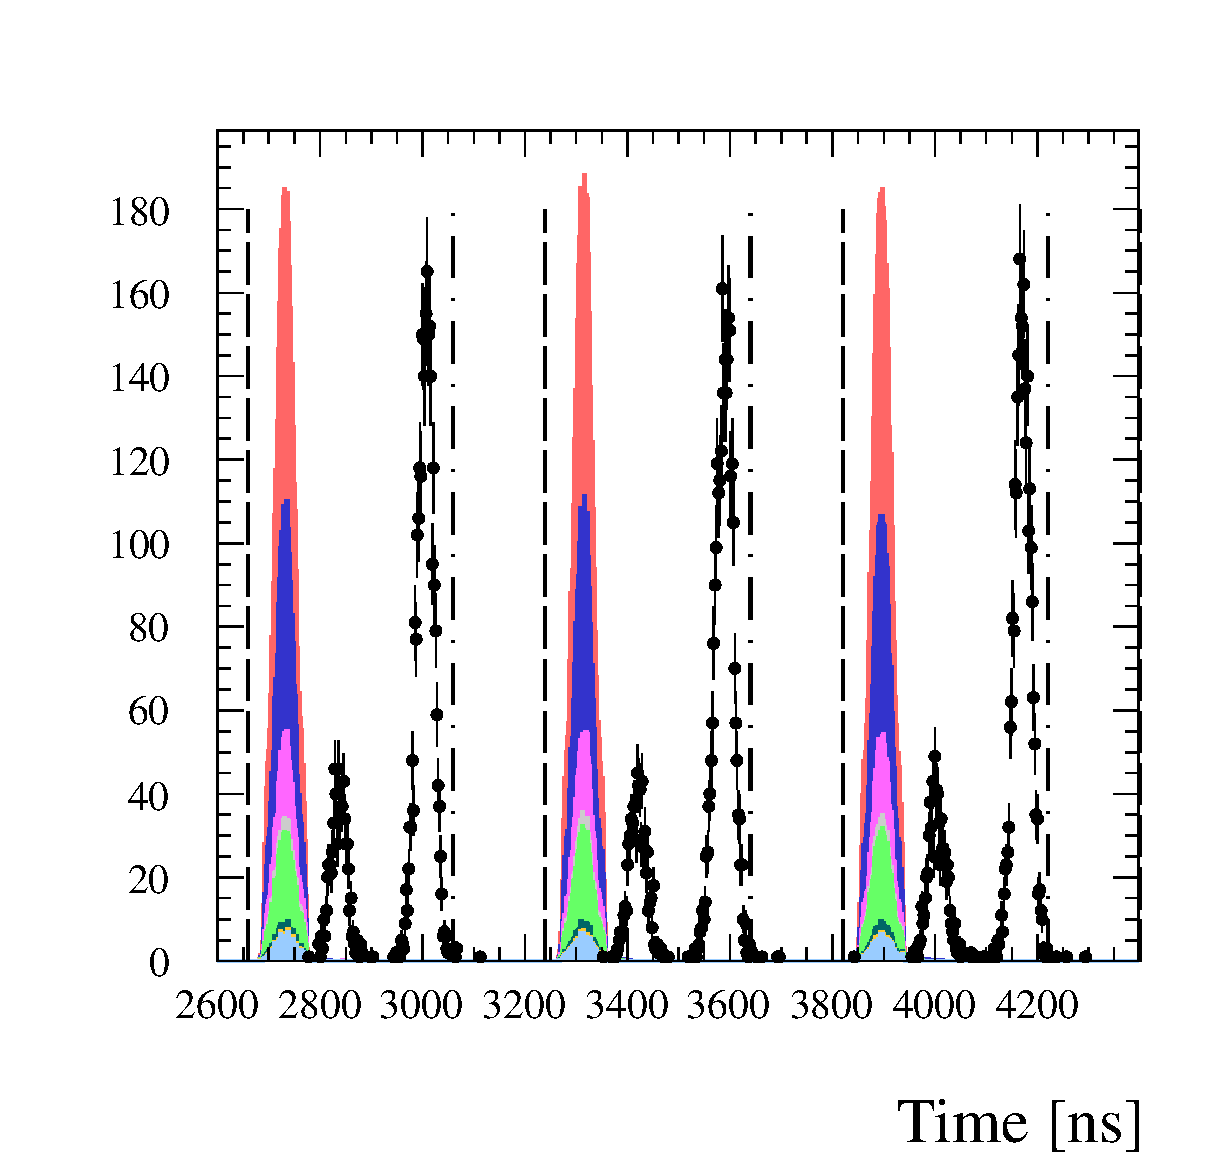
\includegraphics[width=3in]{Figures/P0DTrkTimeRun1Run2Run4-zoom.eps}
\caption{Time distribution of track vertices in Run 1 + Run 2 + Run 4. 
The MC is shown in color and the data in black crosses. 
The left plot shows all the beam bunches and the right plot show a zoom 
in of the first three beam bunches.}
\label{fig:run1time}
\end{figure}

The distribution of 'Water-in' track vertex time in Run 1, Run 2 and Run 4 
is shown in Figures \ref{fig:run1time}. 
We note that there is a discrepancy between the MC track time 
and the Data track time. 
Specifically, the peaks of MC and Data are shifted within the time window. 
%Also, the MC distribution shows a double peaked structure. These effects persist across both running periods with an added structure in the Run 2 data plot. Namely, we see thatin Run 2 there is a second peak in the track timing distribution of Data. 
These effects are not however much of an issue in our analyses as we have very lenient timing cuts. The relative position of peaks in a given time window has a negligible effect when we integrate over the entire window. Any effects at the edge of the timing cuts will be accounted for in our timing systematic.

\subsubsection{Vertex distributions}

We define the start position of the muon candidate track as the vertex. This start position is determined by \p0d reconstruction and corresponds to the first \p0dule to have an above-noise energy deposition from the charged track. For the Z-direction, this implies that the position can only be resolved up to the thickness of an individual \p0dule. The Z Vertex distributions have thus been binned by \p0dule thickness, a value that varies over the different super\p0dules. In the X and Y directions, though we can only get energy deposition in the discrete volumes of scintillator bars, the triangular shape of the bars allows most charged tracks to deposit energy into neighboring bars. The locations of these two hits and the amount of energy deposited at each can be averaged to give a more accurate measurement of where the track passed through the scintillator layer. Thus, the X and Y vertex positions can be resolved to a much higher precision than the Z position.

\begin{figure}
  \centering
  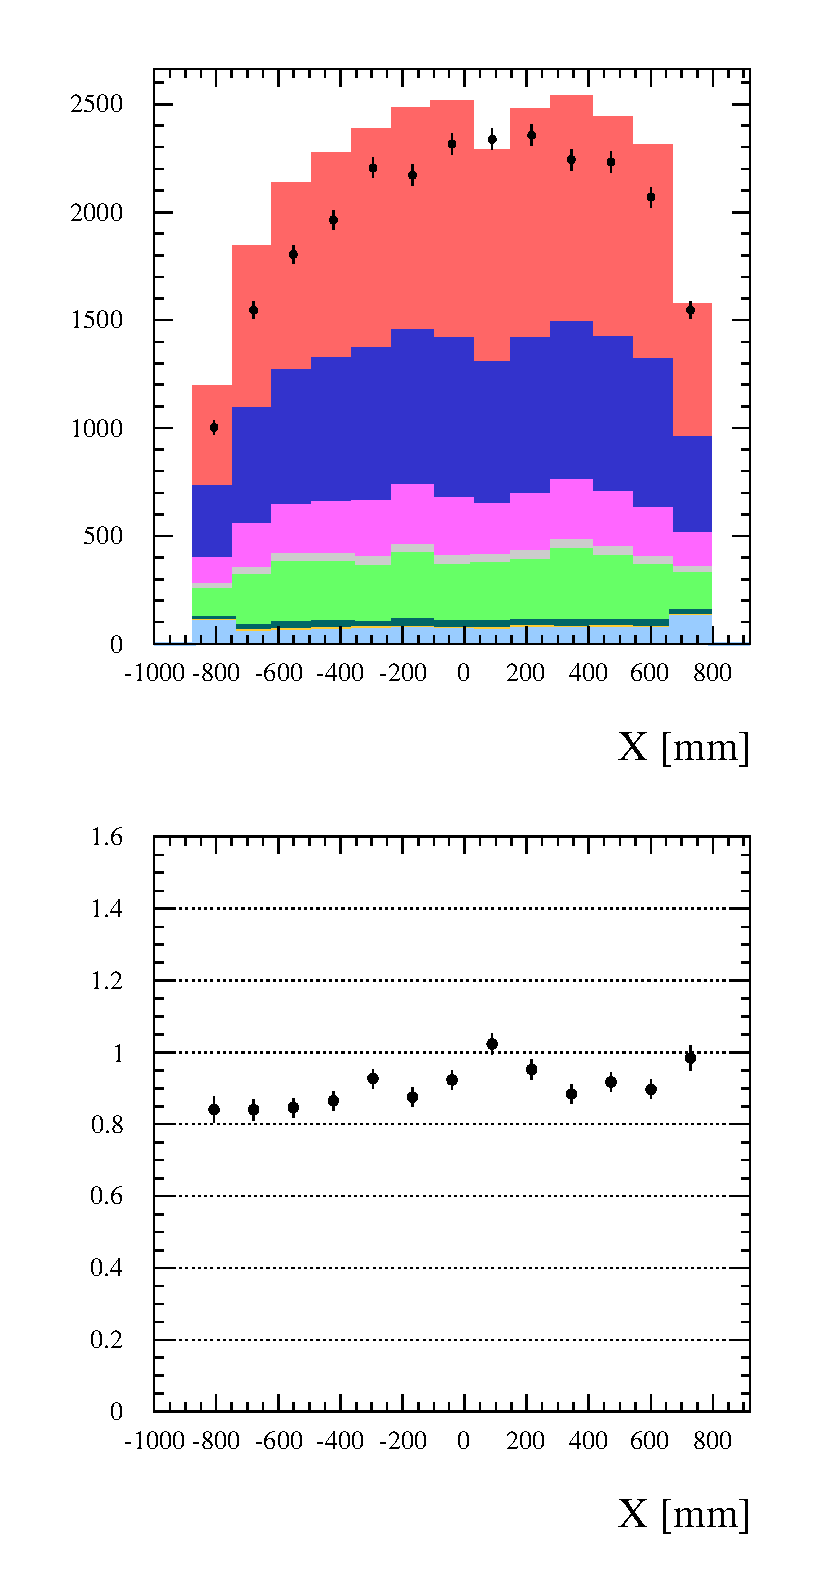
\includegraphics[width=3in]{Figures/P0DTrkXRun1Run2Run4.eps}
  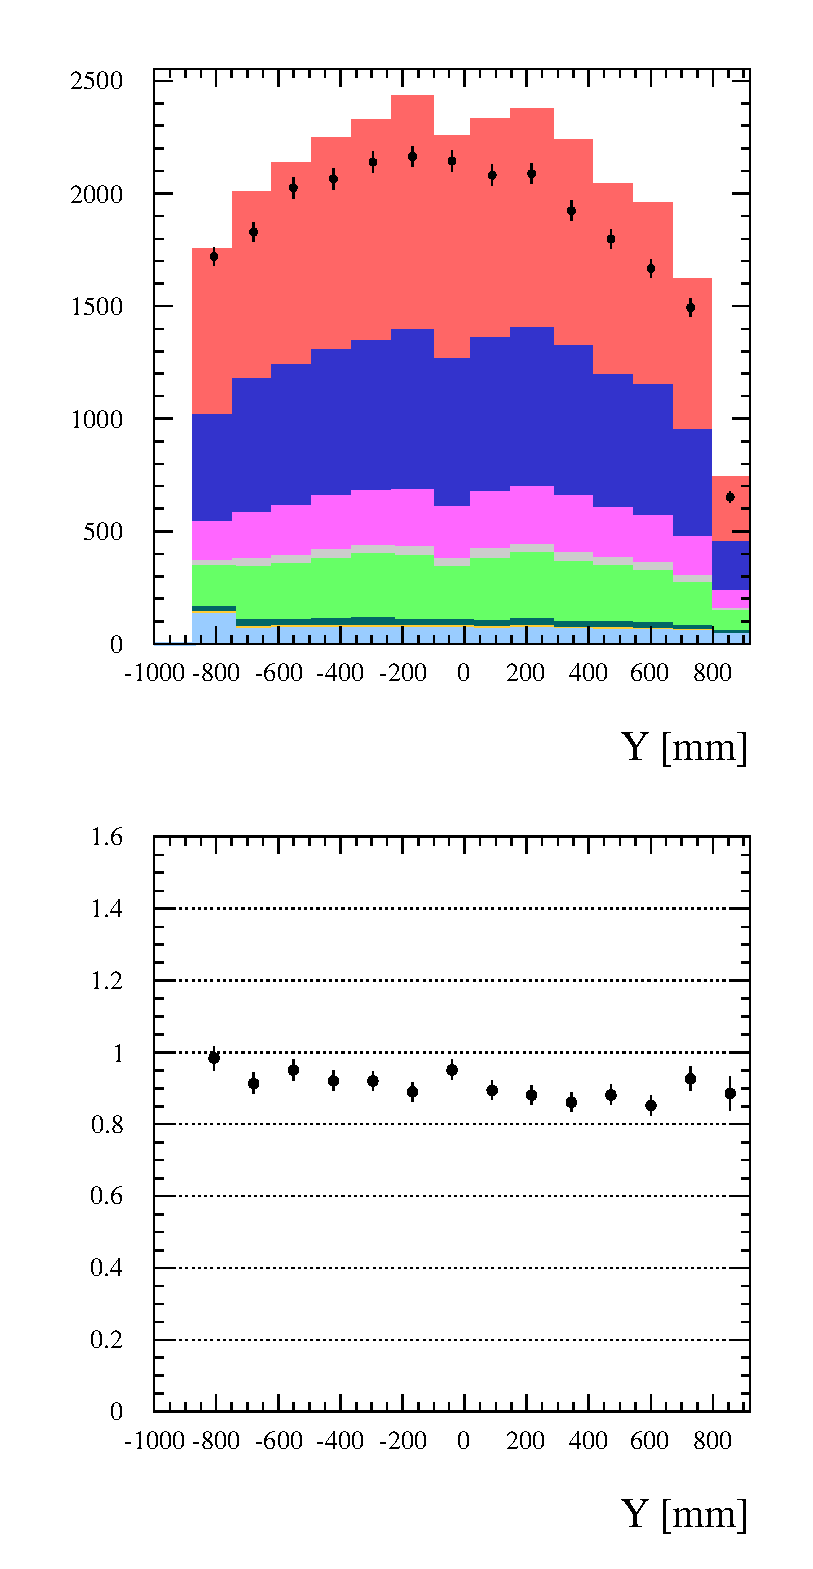
\includegraphics[width=3in]{Figures/P0DTrkYRun1Run2Run4.eps}
  \caption{The start position of the muon candidate track for 
Run 1, Run 2 and Run 4 'water-in' period. The X position (Y position) is shown to the left (right).
Below is the corresponding Data to MC ratio.} 
  \label{fig:XYRun1Run2Run4}%FIXME
\end{figure}

\begin{figure}
  \centering
  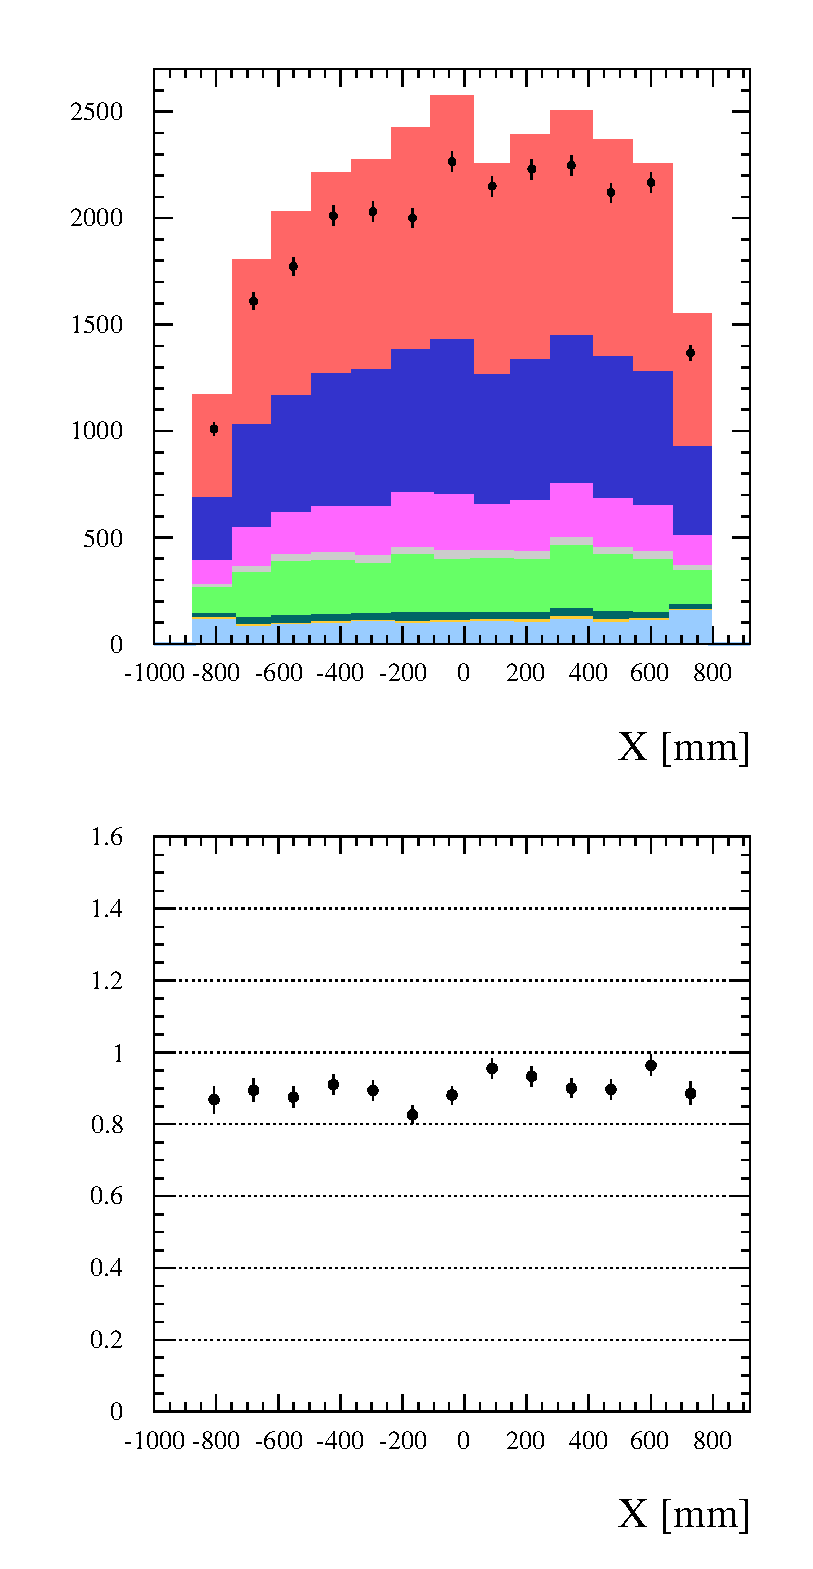
\includegraphics[width=3in]{Figures/P0DTrkXRun2airRun3airRun4air.eps}
  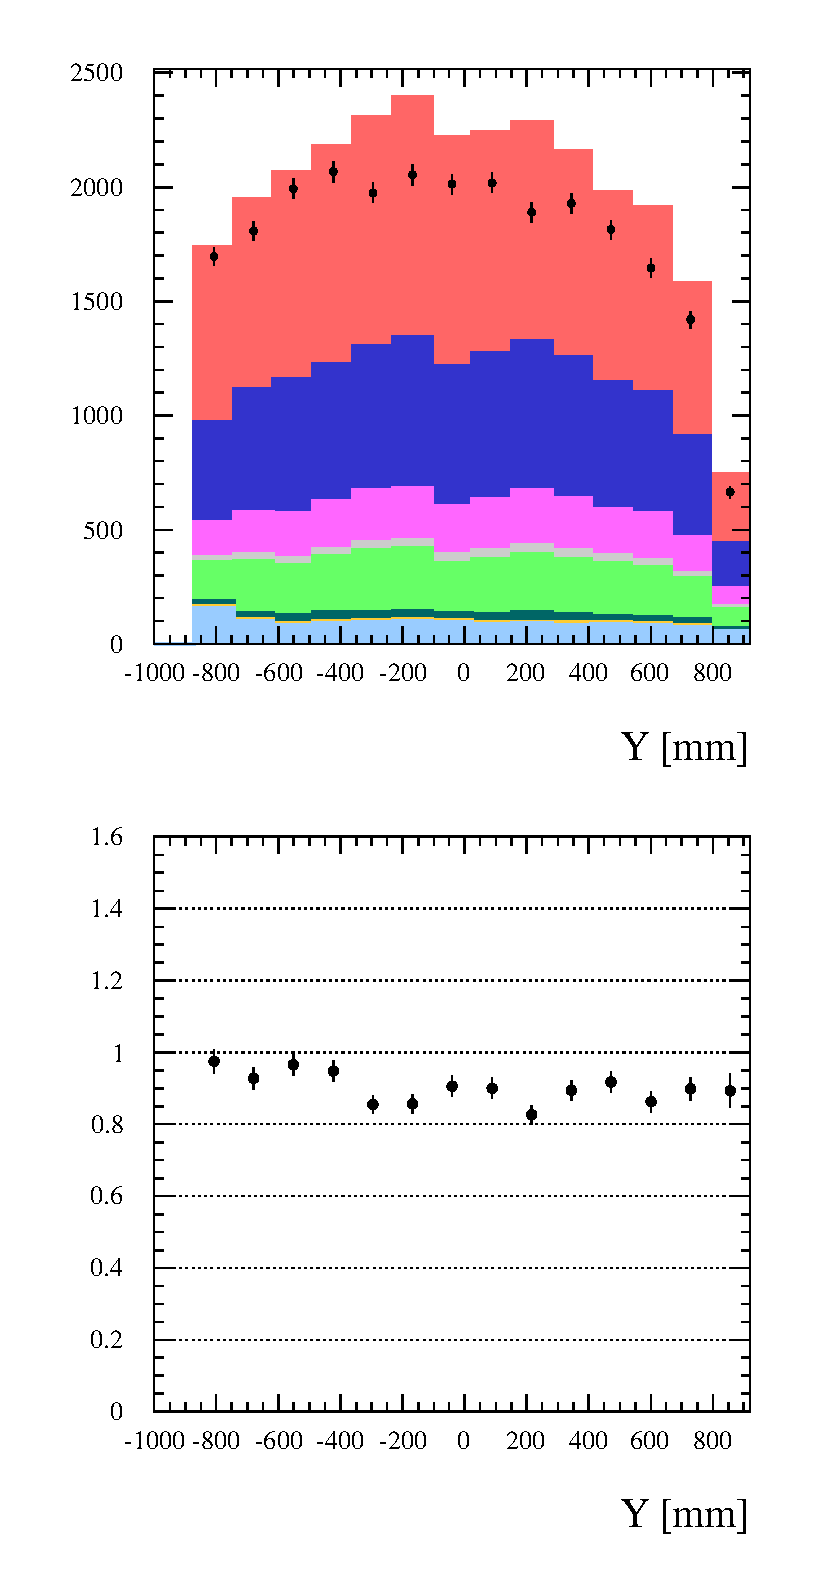
\includegraphics[width=3in]{Figures/P0DTrkYRun2airRun3airRun4air.eps}
  \caption{The start position of the muon candidate track for 
Run 2, Run 3 and Run 4 'Water-out' period. 
The X position (Y position) is shown to the left (right).
Below is the corresponding Data to MC ratio.} 
  \label{fig:XYRun2airRun3airRun4air}%FIXME
\end{figure}

The X, Y and Z vertex positions for the Run 1, Run 2 and Run 4 
'Water-in' periods are shown 
in Figures \ref{fig:XYRun1Run2Run4} and \ref{fig:ZRun1Run2Run4}. 
We note that the number of CC inclusive interactions increases 
as we go further downstream in the \p0d. 
This is an acceptance effect and is expected. 
The muon track candidate must enter the TPC. 
Tracks originating further upstream lose energy 
as they traverse the \p0d and so have  a lower chance of 
making it all the way to the TPC. 
Therefore we see the shape shown in the Z vertex distributions.

\begin{figure}
  \centering
  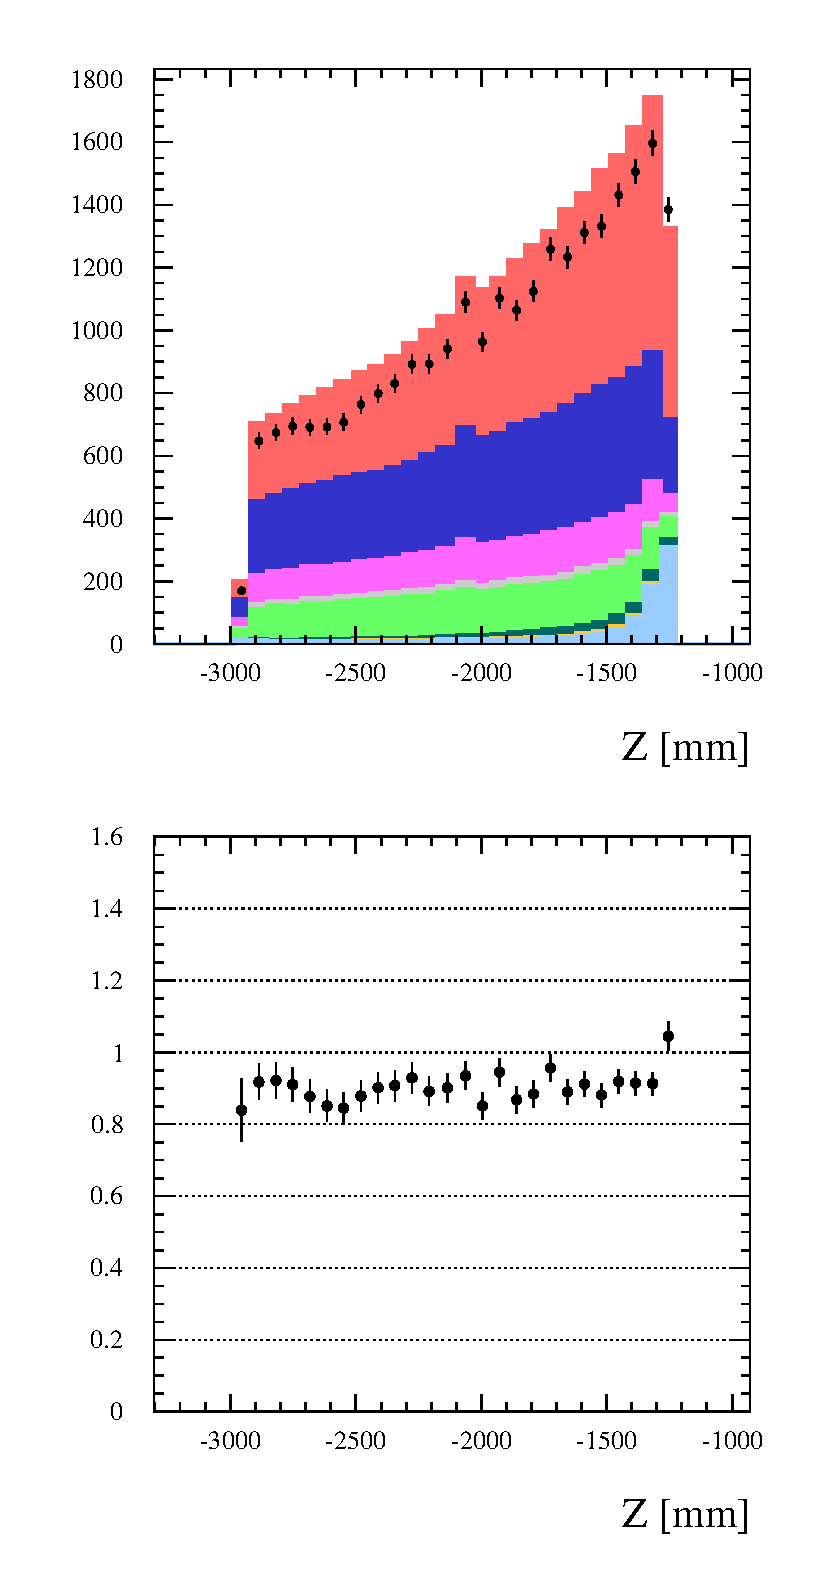
\includegraphics[width=4in]{Figures/P0DTrkZRun1Run2Run4.eps}
  \caption{The Z start position of the muon candidate track for 
Run 1, Run 2 and Run 4 'water-in' periods. 
The varying bin widths equal the thickness of a p0dule in that region. Below is the corresponding Data to MC ratio.} 
  \label{fig:ZRun1Run2Run4}%FIXME
\end{figure}

\begin{figure}
  \centering
  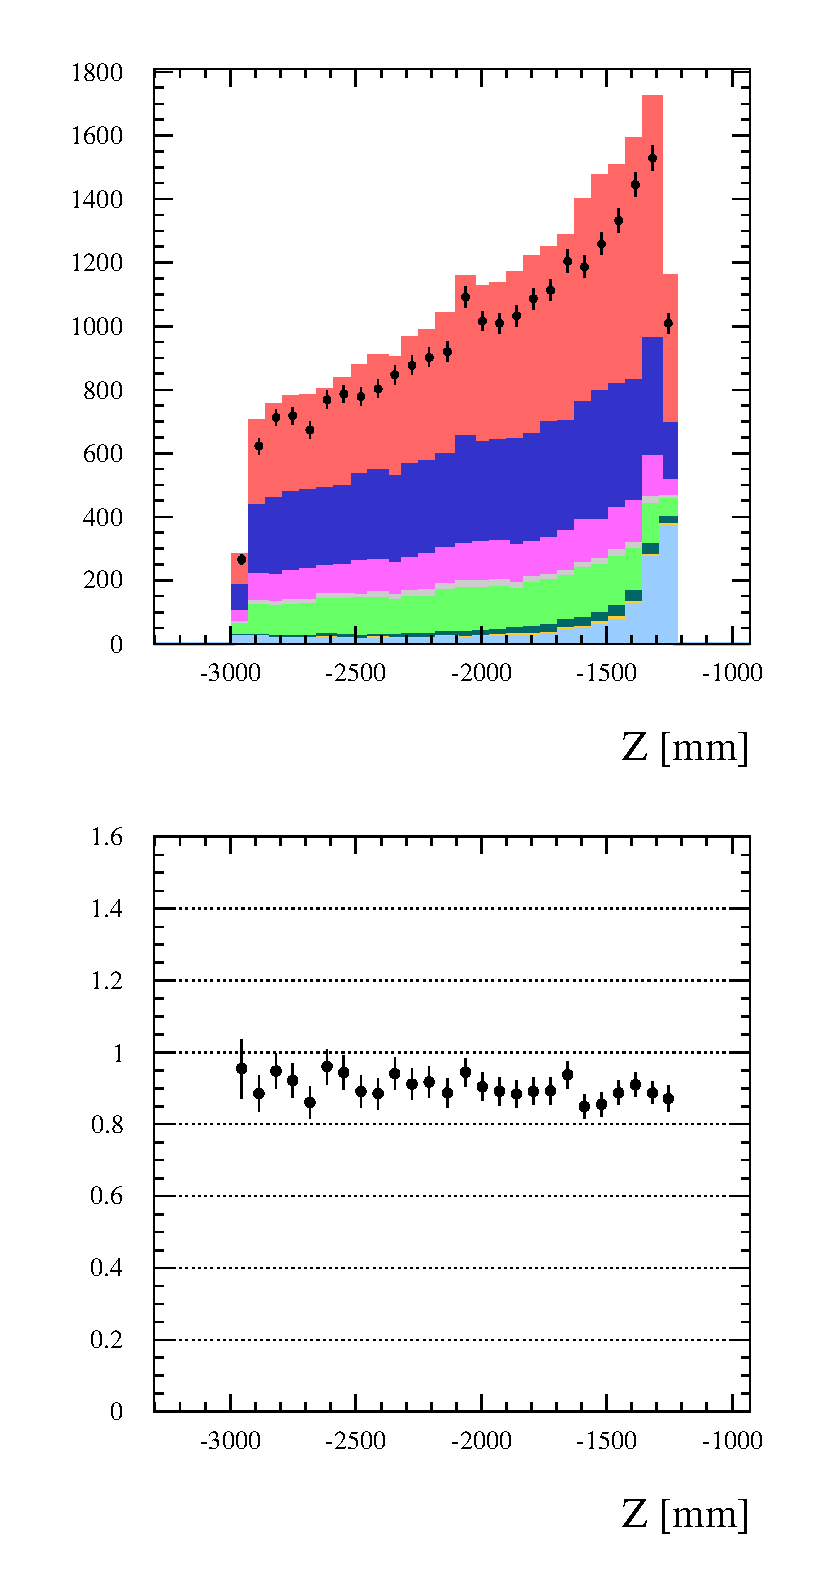
\includegraphics[width=4in]{Figures/P0DTrkZRun2airRun3airRun4air.eps}
  \caption{The Z start position of the muon candidate track for 
Run 2, Run 3 and Run 4 'Water-out' periods. 
The varying bin widths equal the thickness of a p0dule in that region. 
Below is the corresponding Data to MC ratio.} 
  \label{fig:ZRun2airRun3airRun4air}%FIXME
\end{figure}


\subsubsection{Kinematic Distributions}

We show here Data and Monte Carlo distributions of momentum, 
$\theta$ and $\phi$. 
The momentum distributions of the muon candidate tracks 
are shown in Fig. \ref{fig:PmuRun1Run2Run4} for Run 1, Run 2 and Run 4 
'Water-in' periods. 
The markers with error bars represent data with statistical errors 
and the colored histogram stack shows the Monte Carlo separated 
into different interaction categories. 
There is a qualitative agreement in the shape %and normalization 
of the overall momentum distributions between Data and Monte Carlo 
for Run1 + Run2.
 The majority of these background is in the lower momentum region. %Figure \ref{fig:PmuRun1Z} also shows the momentum distribution of the muon candidate track for Run 1 + Run2 respectively. The distributions are also divided into four plots corresponding to the four super\p0dules of the \p0d. The event rate, shape and low energy fall of all agree with what is expected once \p0d energy loss and track acceptance is accounted for.\\
We also show the $\theta$ and $\phi$ distributions of Data and Monte Carlo 
for both running periods. 
Figure \ref{fig:ThetaRun1Run2Run4} indicates that most of our tracks 
are forward going, significantly more so than the FGD selections. 
Once again, this acceptance effect is both expected due to the TPC1 segment 
requirement. 
Figure \ref{fig:ThetaRun1Run2Run4} shows the $\phi$ distribution 
for the combined running periods, and we note good agreement.

\begin{figure}
  \centering
  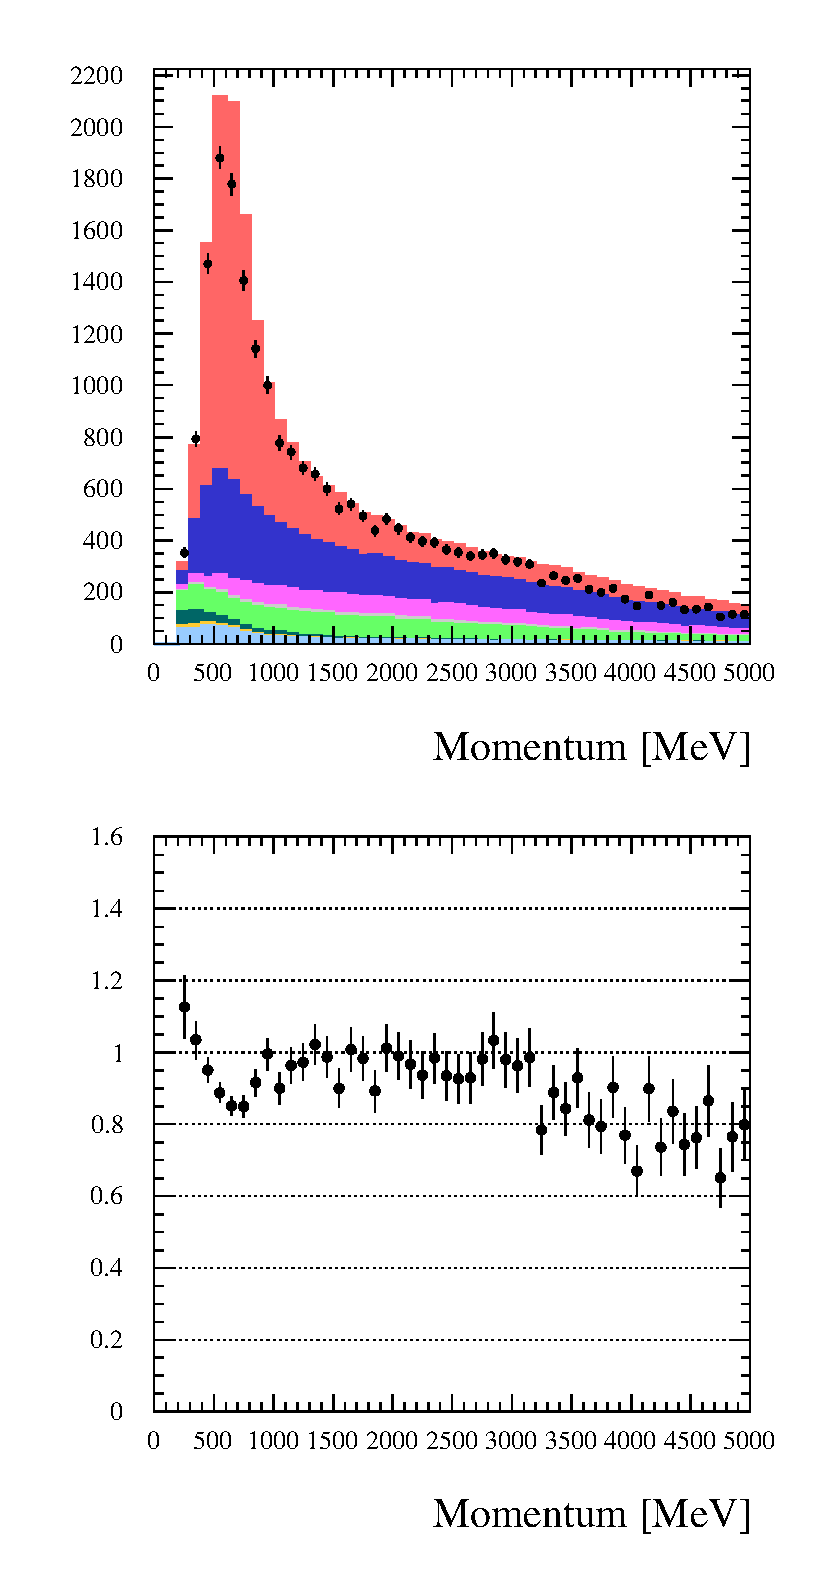
\includegraphics[width=4in]{Figures/P0DTrackerMomRun1Run2Run4.eps}
  \caption{The momentum at the vertex of the muon candidate for 
Run 1, Run 2 and Run 4 'Water-in' peridos. 
Below is the corresponding Data to MC ratio.} 
  \label{fig:PmuRun1Run2Run4}%FIXME
\end{figure}

\begin{figure}
  \centering
  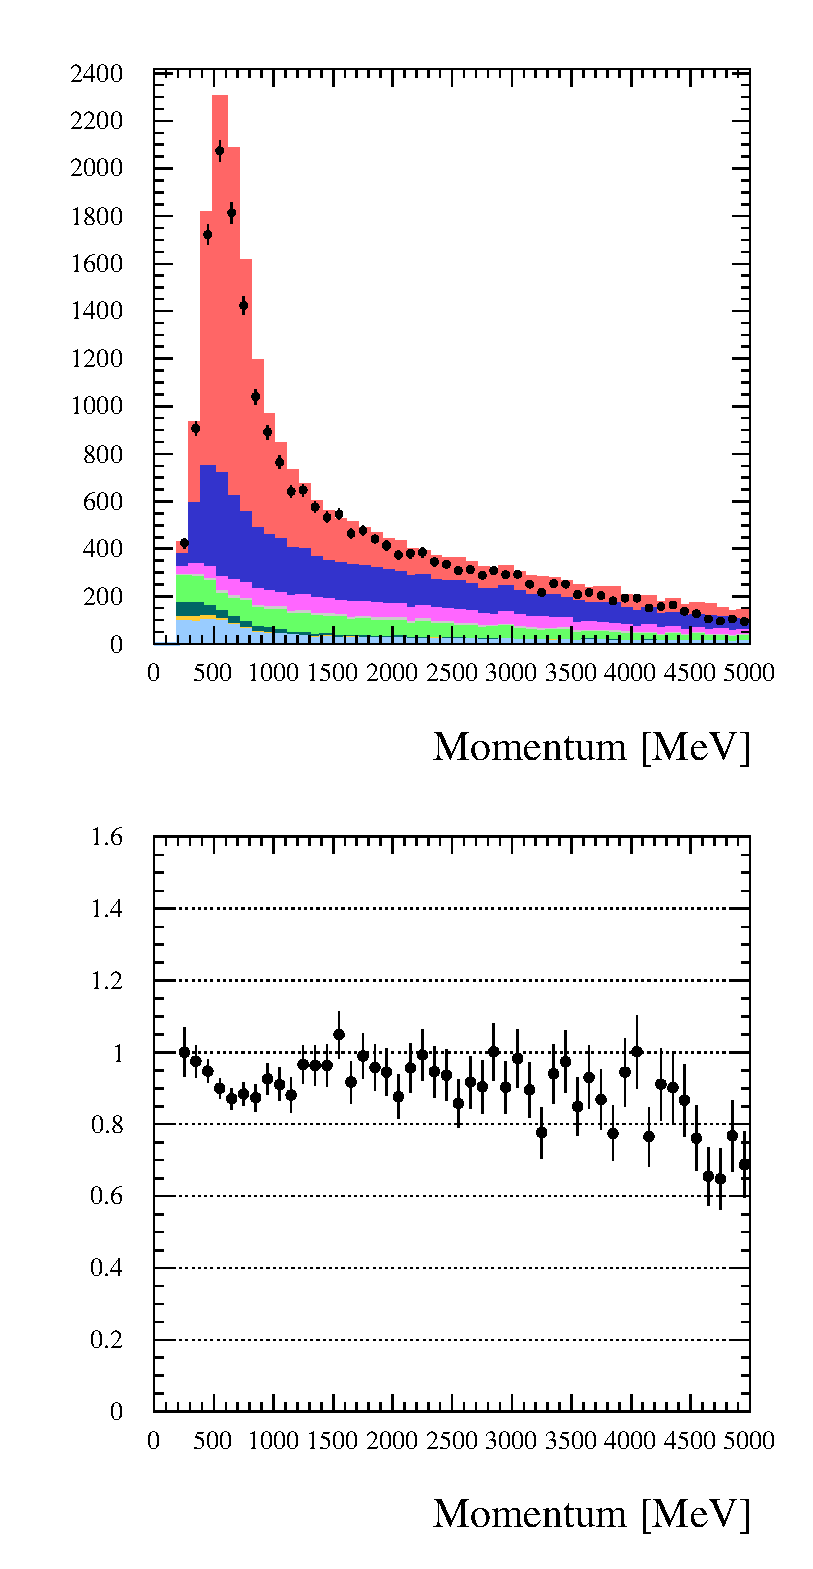
\includegraphics[width=4in]{Figures/P0DTrackerMomRun2airRun3airRun4air.eps}
  \caption{The momentum at the vertex of the muon candidate for 
Run 2, Run 3 and Run 4 'Water-out' peridos. 
Below is the corresponding Data to MC ratio.} 
  \label{fig:PmuRun1Run2Run4}%FIXME
\end{figure}

\begin{figure}
  \centering
  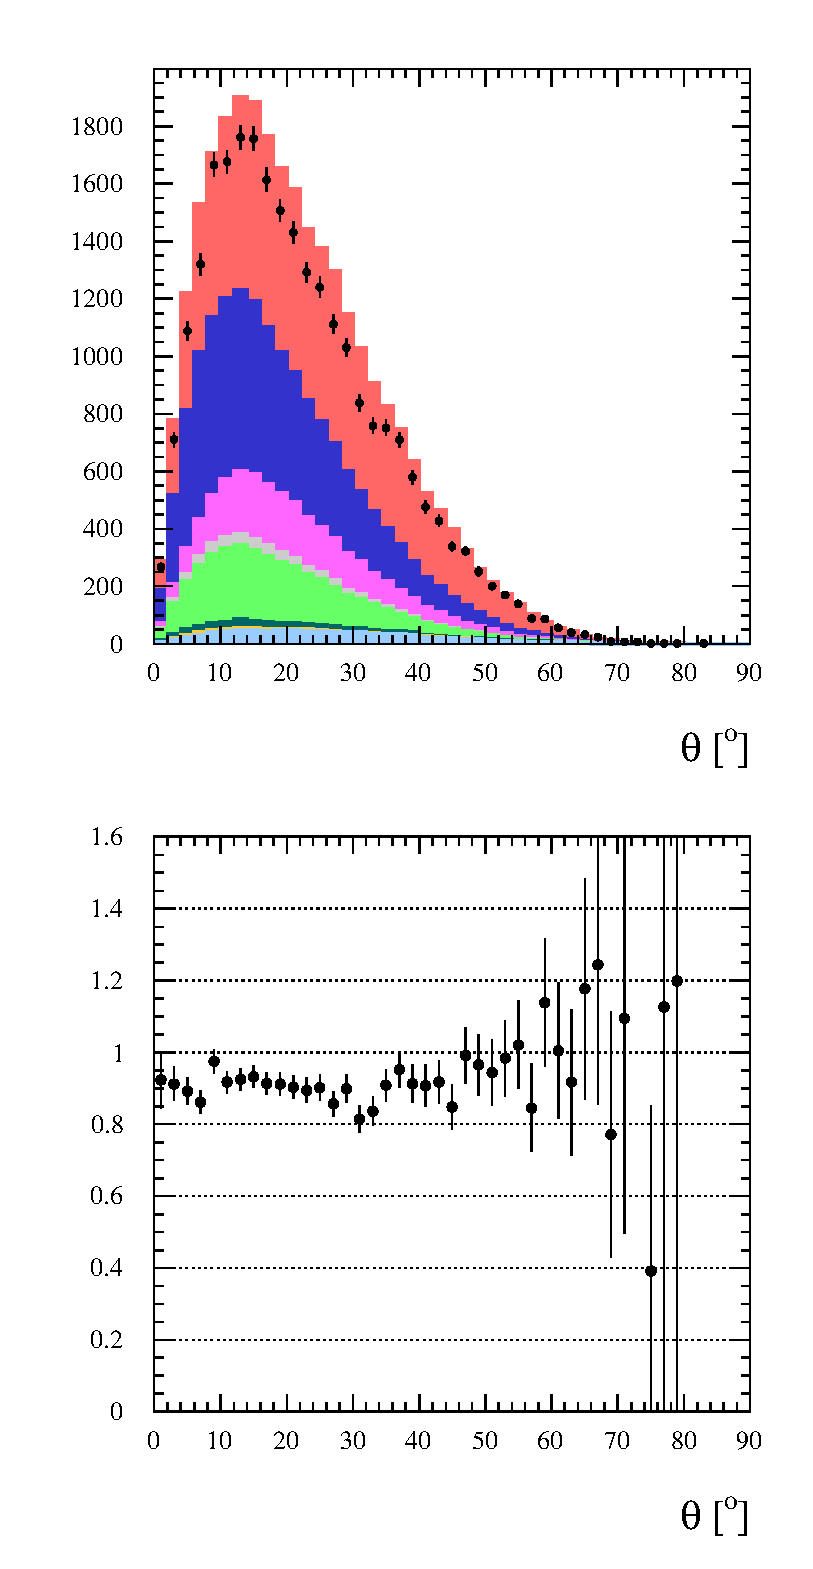
\includegraphics[width=3in]{Figures/P0DTrkThetaRun1Run2Run4.eps}
  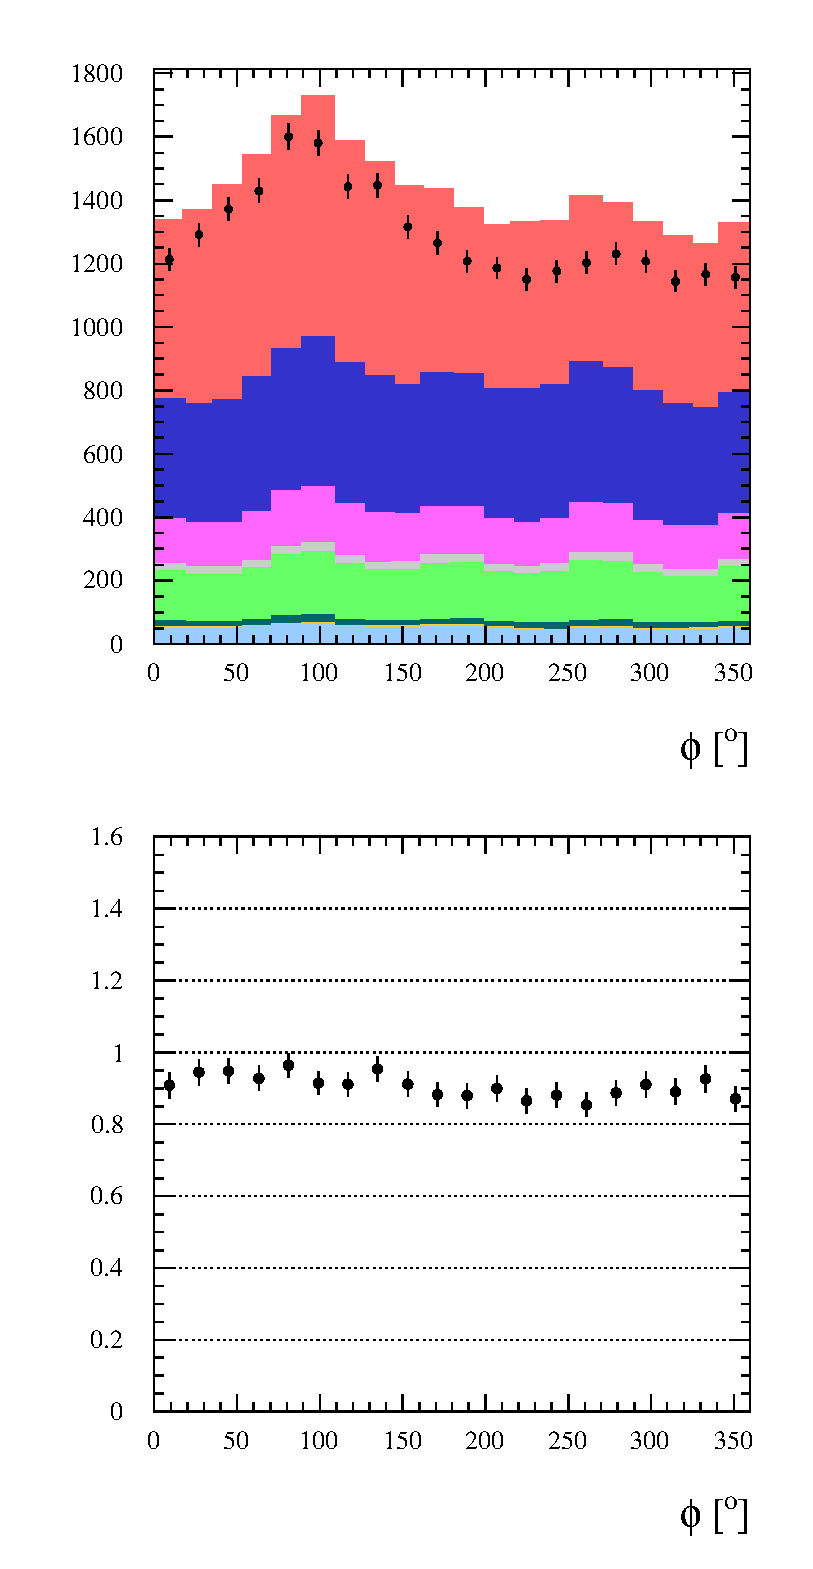
\includegraphics[width=3in]{Figures/P0DTrkPhiRun1Run2Run4.eps}
  \caption{Theta (left) and Phi (right) of the initial direction of 
the muon candidate track in Run 1, Run 2 and Run 4 'Water-in' periods. 
Below is the corresponding Data to MC ratio with statistical errors.} 
  \label{fig:ThetaRun1Run2Run4}%FIXME
\end{figure}

\begin{figure}
  \centering
  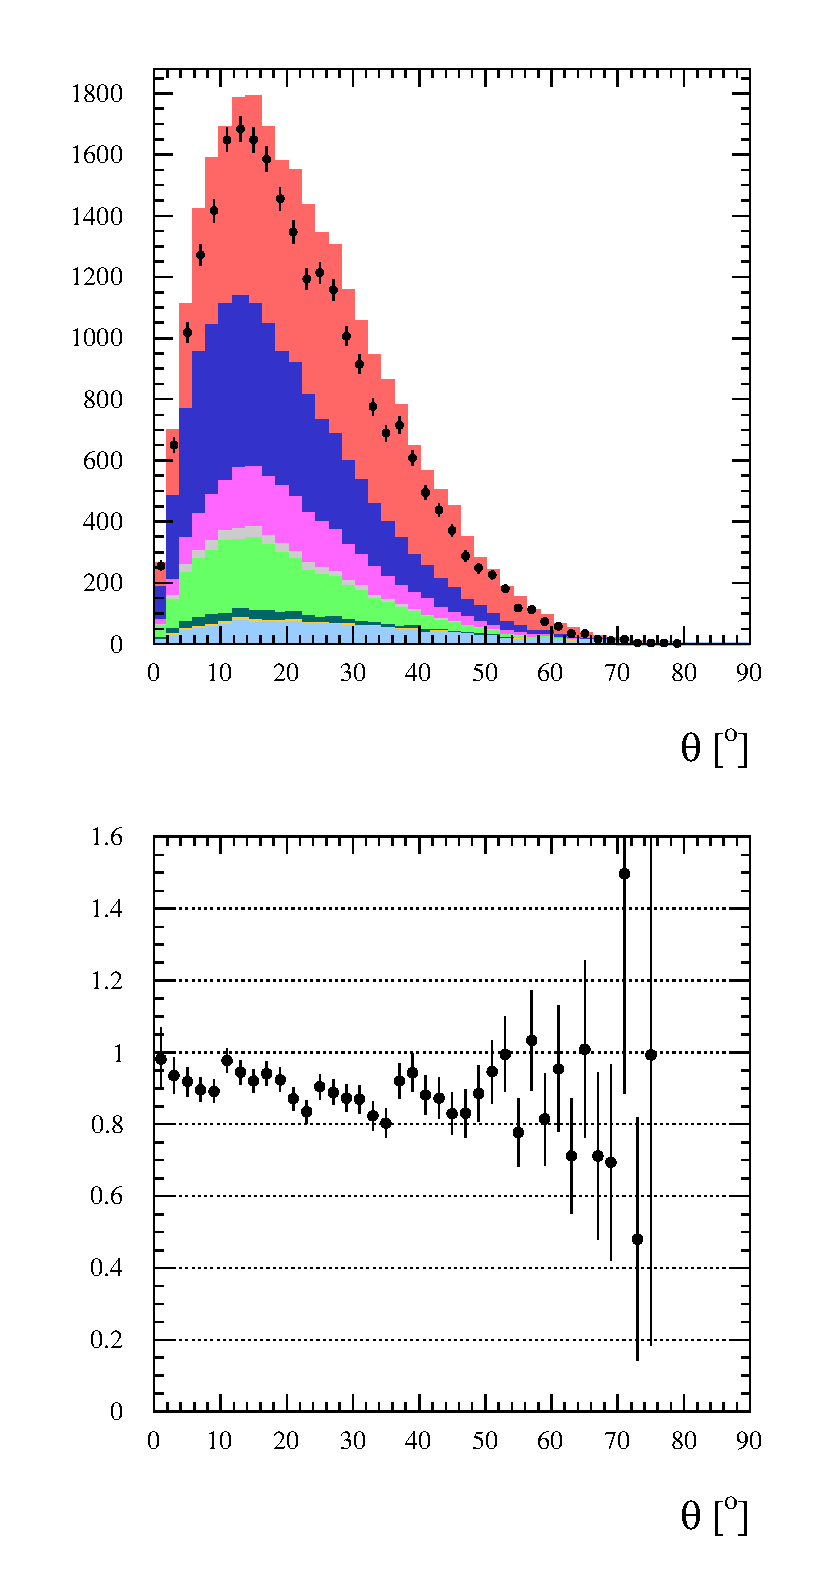
\includegraphics[width=3in]{Figures/P0DTrkThetaRun2airRun3airRun4air.eps}
  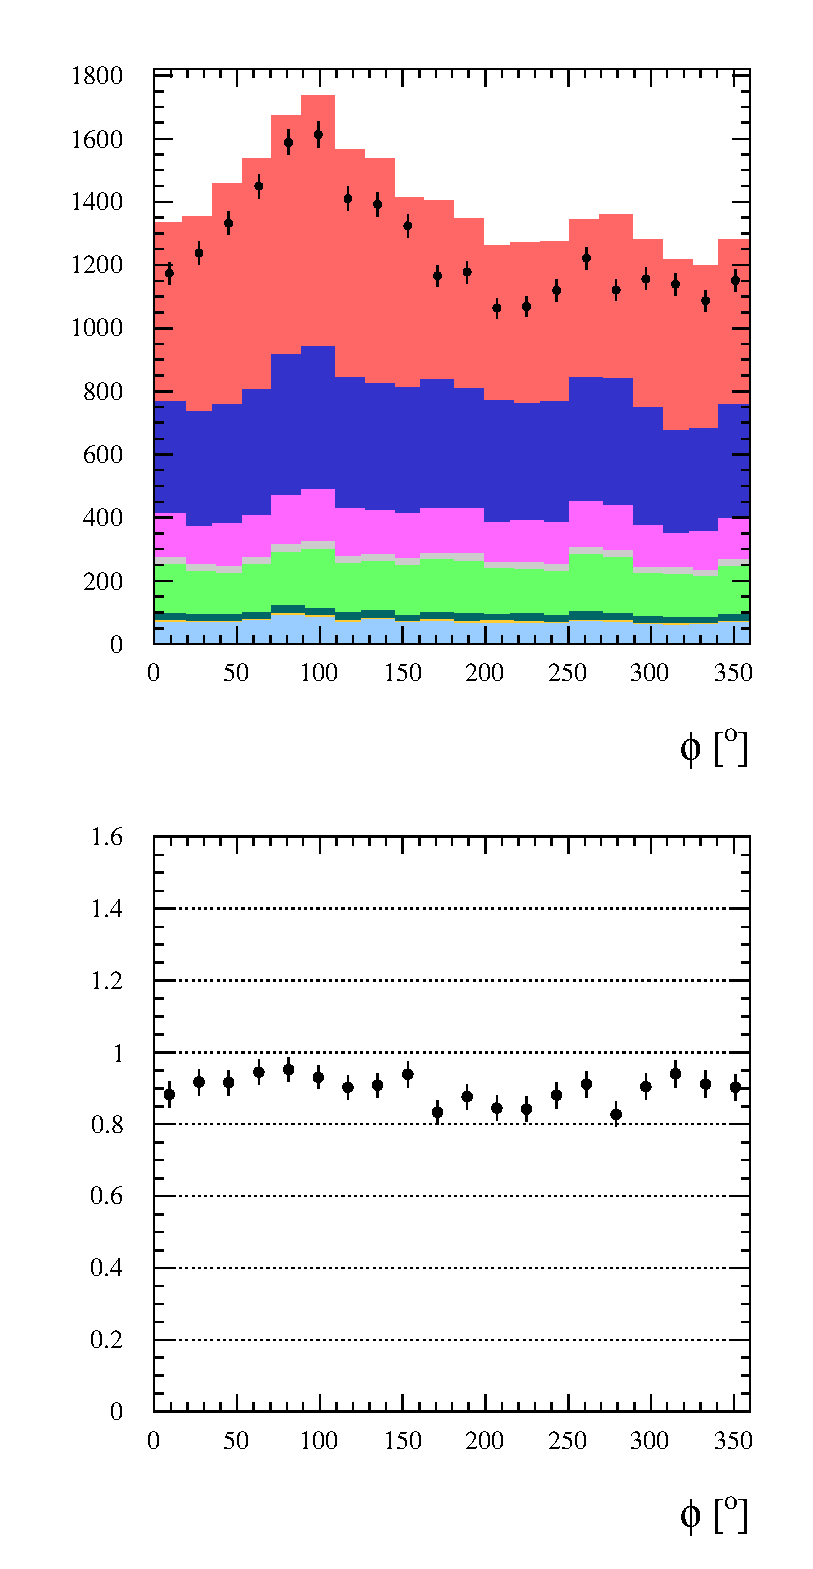
\includegraphics[width=3in]{Figures/P0DTrkPhiRun2airRun3airRun4air.eps}
  \caption{Theta (left) and Phi (right) of the initial direction of 
the muon candidate track in Run 2, Run 3 and Run 4 'Water-out' periods. 
Below is the corresponding Data to MC ratio with statistical errors.} 
  \label{fig:ThetaRun2airRun3airRun4air}%FIXME
\end{figure}

\subsubsection{Results}
\label{sec:RatioResults}

The result is reported as an integrated Data/MC ratio of the total 
selected CC inclusive interactions in Run 1, Run 2 and Run 4 
'Water-in' combined. 
The total events selected in Data is 
25,791 
which corresponds to 
an exposure of $23.6 \times 10^{19}$ POT. 
The unnormalized number of events selected in MC is 
1,031,295
for $626\times10^{19}$ POT. 
After normalizing MC by the Data POT 
and applying the fiducial mass correction (to each of the run periods 
as detailed in TN-073), 
we have yielded the Data/MC ratio of 
$ 0.879 \pm 0.006 $.\\

For completeness we summarized in Table \ref{tab:MCBreakdown} 
the number of events after all normalization and corrections 
for the different MC channels that we selected.

\begin{table}[h]
\centering
\begin{tabular}{lcc}
\toprule
MC Channel & & Number of events selected \\
\cline{1-1}\cline{3-3} 
QE & & 11,895 \\
Pi & & 8,294 \\
NPi & & 3,008 \\
Meason & & 480 \\
DIS & & 3,329 \\
NC & & 381 \\
$\bar{\nu}$ & & 98 \\
Other & & 7 \\
Out of FV & & 916 \\
\bottomrule
\end{tabular} 
\caption{
The number of events selected in the 
CC inclusive MC 
Run 1, Run 2 and Run 4 for the 'Water-in' periods 
combined sample, 
presented for the different MC channels. 
}
\label{tab:MCBreakdown} 
\end{table}

\begin{table}[h]
\centering
\begin{tabular}{lcc}
\toprule
MC Channel & & Number of events selected \\
\cline{1-1}\cline{3-3} 
QE & & 11,956 \\
Pi & & 7,700 \\
NPi & & 2,745 \\
Meason & & 440 \\
DIS & & 3,078 \\
NC & & 427 \\
$\bar{\nu}$ & & 110 \\
Other & & 7 \\
Out of FV & & 1,290 \\
\bottomrule
\end{tabular} 
\caption{
The number of events selected in the 
CC inclusive MC 
Run 2, Run 3 and Run 4 for the 'Water-out' periods 
combined sample, 
presented for the different MC channels. 
}
\label{tab:MCBreakdown} 
\end{table}

\clearpage
